\section{Detektor}\label{sec:detect}
Feature detektion er en metode indenfor billedbehandling, der for hvert punkt $p = (x,y)$ i et billede $I$ bestemmer, om punktet er et interessepunkt. Et interessepunkt kan karakteriseres som\cite{pointsurvey}:
\begin{itemize}
\item{\emph{Repeterbar}: Repeterbarheden significere uafhængighed af forskellige betingelser i billedet. Dvs. at samme interessepunkt skal kunne findes i to forskellige billeder, trods ændringer af f.eks lys og rotation}
\item{\emph{Distinktive:}
Intensiteten i og omkring interessepunktet skal være unikt, så et interessepunkt er entydigt lokaliserbart}
\end{itemize}
En feature detektor '$Detect$' er en funktion, der tager et billede som input, og returnere interessepunkter.
\begin{equation}
Detect(I)= \bold{P}
\label{detect}
\end{equation}
hvor $P = {p_1, p_2,..., p_n}$.
Moravec \cite{moravec} definerer som en af første et brugbart interessepunkt således: "A
feature is good if it can be located unambiguously in different views of a scene. A
uniformly colored region or a simple edge does not make for good features because
its parts are indistinguishable. Regions, such as corners, with high contrast in
orthogonal directions are best." I følge Moravec, indeholder et godt interessepunkt en stor kontrast, i de ortogonale retninger. Der findes mange definitioner af et interessepunkt, og i sidste ende angiver anvendelsesområdet, hvilke punkter, der lokaliseres bedst.
\begin{figure}[H]
    \centering
    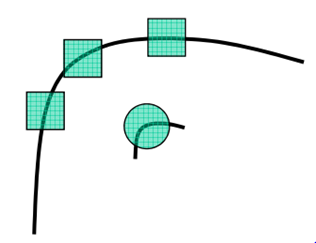
\includegraphics[width=0.37\textwidth]{fig/28.png}
     \vspace{-1em}
    \begin{center}    
       \caption{\textcolor{gray}{\footnotesize \textit{To ens kurver, set på forskellige to To ens kurver, set på forskellige skalaer. Opfattes kurven langt væk, som den store kurve, vil de udvalgte områder opfattes som kanter. Opfattes hele kurven vil området vise et hjørne. Det kan derfor, alt efter applikationsdomænet, være nødvendigt at anvende en skala invariant detektor.}}}
    \label{fig:skal}
     \end{center}
     \vspace{-2.5em}
  \end{figure} \noindent
En Detektor skal være robust overfor små deformationer som støj (tilfældig intensitetsvariation, der ikke er tilstede i scenen) i billedet, hvilket fejlagtigt kan fortolkes som interessepunkter. Imellem to billeder, kan der være geometriske forskelligheder, som f.eks. rotation, skalering(se figur  \ref{fig:skal}) ændring af perspektiv. Der kan også forekomme fotometriske ændringer, som ændring af pixelintensitet forsaget af lysændringer. Disse faktorer, skal en detektor helst være invariant overfor.  
\\
\\
Interessepunkter defineres ikke udfra semantisk meningsfulde områder, som ansigter eller bøger, da dette vil kræve en høj-niveau fortolkning af scenen. I stedet anvendes lav-niveau strukturere, der identificeres i lokale pixelområder, og er matematisk definerbare. Nedenstående er en gennemgang af forskellige lokale lav-niveau strukturere, der kan bruges i udvælgelsen af interessepunkter.
\newpage
\subsection{Hjørner}\label{subsec:corner}
At detektere hjørner er en udbredt teknik indenfor feature detektion, da hjørner ofte forekommer i forskellige menneskeskabte scener og fordelagtigt kan bruges i disse sammenhæng. Et hjørne kan defineres som et område i og omkring et punkt, der har to dominerede kantretninger og kan derved lokaliseres i et billede udefra en kvantificeret fortolkning af dette. \\ Udover at være lokaliserbare ved en matematisk definition, skal et interessepunkt besidde en unik struktur, der tillader en entydig korrespondance. I figur \ref{app} ses tre udvalgte punkter, placeret forskelligt i samme scene, hvor punkterne beskrives af en blå cirkel omkring punktet. Figuren illustrere mulige korresponderende punkter, for et givent interessepunkt.
\begin{enumerate}[label=\alph*]
\item{Interessepunktet er placeret på et fladt området, hvor intensiteten er ens for hele området. Punktet vil have mange mulige korresponderende punkter.}
\item{ Interessepunktet er lokaliseret på en kant. Punktet vil have flere mulige korresponderende punkter på den tilsvarende kant i den anden figur.}
\item{Interessepunktet er lokaliseret på et hjørne. Det ses at kun ét andet punkt i modsvarende scene er identisk med dette.}
\end{enumerate}
\begin{figure}[H]
    \centering
    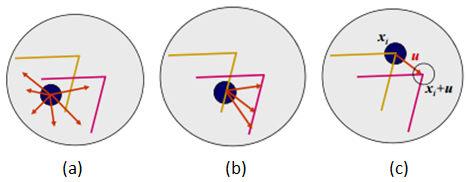
\includegraphics[width=0.55\textwidth]{fig/37.png}
    \vspace{-1em}   
    \begin{center}    
    \caption{\textcolor{gray}{\footnotesize \textit{
 }}}
    \label{app}
     \end{center}
    \vspace{-2.7em}  
  \end{figure}  
\noindent
Ovenstående definition viser at punkter placeret på hjørner er unikke og kan derfor entydigt differentieres fra ikke korresponderende punkter. Hjørner kan som nævnt udvælges i billederne pga. de dominerende kantretninger i og omkring punktet, hvilket medfører store intensitetsskift i området omkring et hjørne. En af de første hjørne detektorer udviklet af Moravec \cite{Moravec} lokalisere et hjørne ved at estimere auto-korrelationen imellem regioner af billedet, og definere hjørner, hvor der forekommer store intensitetsskift omkring et punkt.
\chapter{Metoder indenfor billedbehandling}\label{subsec:kant}
Formelt kan et gråtonebillede repræsenteres som en funktion af to variable:
\begin{equation}
\begin{split}
&I: \mathbb{\mathbb{Z^+}}^2 \rightarrow \mathbb{Z}^+ \\
&I(x,y) = \lambda_{x,y} \hspace{0.5 cm} (x,y)\in \mathbb{Z^+}^2, \lambda_{x,y} \in [1,256] \subset \mathbb{Z^+}
\end{split}
\label{bf}
\end{equation}
hvor $\lambda_{x,y}$ repræsentere en billedintensitet, også kaldet en pixelværdi. $\lambda_{x,y}$ er defineret, indenfor grænserne af billedet og er 0 udenfor, dvs.: 
\begin{equation}
 I(x, y) =
\begin{cases}
    \lambda_{x,y}, & \text{hvis } 1 \leq x \leq x_{max}, 1 \leq y \leq y_{max} \\
    0,              & \text{ellers}
    \label{pixelintensitet}
\end{cases}
\end{equation}
En kort bemærkning bør gøres om det anvendte billedformatet. De undersøgte billeder er af filtype JPEG(Joint Photographic Experts Group) og hver pixelintensitet indeholder originalt 8x3 bits information til hhv. rød, grøn og blå: $\Lambda_{x,y} = [R,G,B]^T \in \mathbb{R}^3$. Hver farve kan antage $2^8 = 256$ forskellige værdier og hver værdi ligger i intervallet $[0,1]$. Disse værdier bliver transformeret til en gråtoneværdi:
\begin{equation}
Lum(\Lambda_{x,y}) = \lceil	 256 \cdot [0.299, 0.587, 0.114] \Lambda_{x,y} \rfloor	 = \lambda_{x,y}
\label{lumosity}
\end{equation}  
Hver gang pixelværdi eller billedintensitet benævnes, er det underforstået, at de har undergået den lineære transformation, ligning \eqref{lumosity}. I denne opgave håndteres kun gråtonebilleder, derfor er ligning \eqref{lumosity} brugt til at transformere RGB billeder til gråtone billeder \footnote{I Python er biblioteket cv2 anvendt. Transformationen fra RGB til gråtone dokumenteret her %\url{<http://docs.opencv.org/2.4/modules/imgproc/doc/miscellaneous_transformations.html>}. 
Denne transformation bliver nærmere beskrevet i \cite{lumosity}. en uddybning og alternativer kan læses i afsnit 7.6} 
\\
\\
Ofte i billedbehandlings situationer betragtes diskontiniuteter i billedet, f.eks. kanter.
Hvis et billede beskues i 3D, kan en kant illustreres i 1D, ved et snit af et billede vinkelret på fladen i gradientens retning, illustreret i figur \ref{fig:kant}. En kant er en lokal ændring i det afledte signal $f$.
\noindent
\begin{figure}[H]
    \centering
    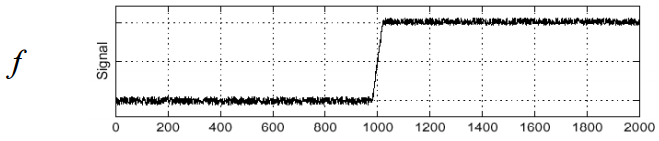
\includegraphics[width=0.55\textwidth]{fig/7.png}
     \vspace{-1em}
    \begin{center}        
     \caption{{\footnotesize \textit{
En 1-dimensional fortolkning af intensiteten i et billede. Intensitetsskiftet i midten (ved x $\approx$ 1000, er en kant.)}}}
    \label{fig:kant}
     \end{center}
       \vspace{-2.5em}
  \end{figure}
\noindent
En differentiering af funktionen fra figur \ref{fig:kant} en stigning i pixelintensiteten  og derved angive hvor der forekommer kanter. Differentiering af billeder kan f.eks. approsikmeres ved følgende ligning:
\begin{equation}
\dfrac{df(x)}{dx}=\dfrac{f(x+1)-f(x-1)}{2}
\label{diff}
\end{equation}
Foldning er en operation, der indenfor billedbehandling bruges til modificere et billede. Modificeringen kan f.eks. være sløring, fokusering eller fremhævning af visse strukturer. Foldning af $I$ af størrelse $(M \times N)$, med en kerne $K$, der har størrelse $(k \times l)$, hvor $M > k, N > l$, angives ved:
\begin{equation}
O(i,j) = \sum_{k} \sum_{l} I(i-k, j-l) K(k,l)
\label{foldning}
\end{equation}
Ligning \eqref{foldning} udregnes for alle $i,j \in I$. En kerne defineres her som en matrix af arbitrær dimension - ofte $(N\times N)$. 
\\
\\
Et billede kan differentieres, som anført ligning \eqref{diff}, ved brug af foldning. Først defineres en kerne til differentiering i $x$-aksen $K$, som: $K = [\frac{1}{2}, 0, \frac{1}{2}]$. Kernen foldes med billedet $I$: $I \ast K $, hvor $\ast$ udgør foldningsoperatoren. Når en kerne skal foldes med et billede hvor afstanden til randen af billedet er skarpt mindre, end størrelsen af kernen, gælder ligning \eqref{pixelintensitet} for $I$.
\\
\\
Det kan være problematisk at lokalisere kanter vha. differentiering. I figur \ref{fig:kant}, vil støj i billedet(de små udsving) også blive fremhævet. For at fjerne støjen, kan billedet foldes med et Gaussisk filter, hvilket er en diskret approksimering til den Gaussiske funktion. Foldning af et billede med et Gaussisk filter vil resultere i en flydende overgang af pixelværdierne og derfor glatte billedet. <sæt gaussbillede ind> Den Gaussiske funktion i 2-D, hvor $ \sigma $ er standardafvigelsen af den Gaussiske fordelingen, er defineret som:
\begin{equation}
G(x,y,\sigma) = \frac{1}{2 \pi \sigma ^{2}} e^{- \frac{x^{2} + y^{2}}{2 \sigma ^{2}}}
\label{2dgaussian}
\end{equation} 
For at undgå først at glatte billedet ved at folde med et Gaussisk filter, og derefter folde med et differentieringsfilter udnyttes det, at foldning er en associativ operation:
\begin{equation}
\dfrac{\partial}{\partial x}(G \ast f) = (\dfrac{\partial}{\partial x}G) \ast f
\end{equation}
Her er $G$ er det Gaussiske filter, men kunne være en vilkårlig anden kerne, og $f$ et signal. 
\\
Foldes et differentieret 1-dimensionelt Gaussfilter med signalet fra figur \ref{fig:kant}, vil det resultere i et bakkeformet signal, hvor maksima af bakken indikere en kant, dette er illustreret i figur \ref{fig:firstd}.
\begin{figure}[H]
    \centering
    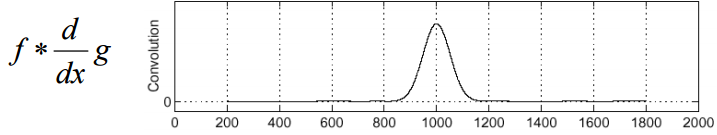
\includegraphics[width=0.55\textwidth]{fig/100.png}
     \vspace{-1em}
    \begin{center}        
     \caption{{\footnotesize \textit{
Signalet fra figur \ref{fig:kant} foldet med et første afledt Gaussisk filter.)}}}
    \label{fig:firstd}
     \end{center}
       \vspace{-2.5em}
  \end{figure}
\noindent
For en mere lokaliserbar kant, kan den dobbelt afledte tages, som set i figur \ref{fig:deriv}. I sidstnævnte tilfælde, kan kanten lokaliseres, hvor funktionen krydser nul.
\begin{figure}[H]
    \centering
    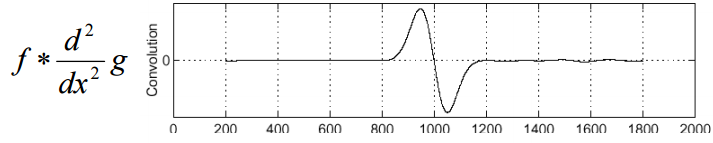
\includegraphics[width=0.55\textwidth]{fig/101.png}
    \vspace{-1em}   
    \begin{center}
    \caption{{\footnotesize \textit{
     Resultatet af at folde et dobbelt differentieret Gaussisk filter med funktionen fra figur \ref{fig:kant}.}}}
    \label{fig:deriv}
     \end{center}
    \vspace{-2.5em}  
  \end{figure}
\noindent
I de anvendte metoder er der blevet gjort brug af et dataindsamlingsvindue. Med dette menes et udsnit af et billede, omkring et punkt. Figur \ref{fig:dataindvin} illustrerer et dataindsamlingsvindue omkring $I(3,4)$, der har størrelsen $(3 \times 3)$. Det skal bemærkes, at et dataindsamlingsvindue i denne opgave også kan bestå af andre værdier end pixelintensiteter. Det indeholder også gradient størrelse og gradient retninger.
\begin{figure}[H]
    \centering
    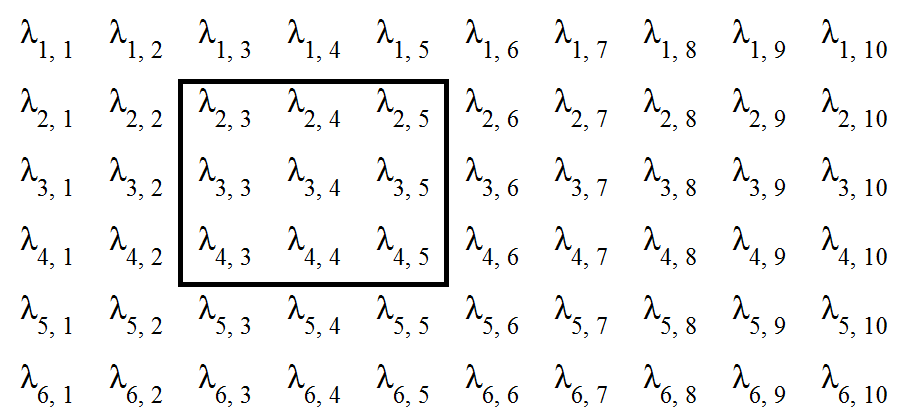
\includegraphics[width=0.55\textwidth]{fig/dataindsamlingsvinduepic.png}
    \vspace{-1em}   
    \begin{center}
    \caption{{\footnotesize \textit{
     Resultatet af at folde et dobbelt differentieret Gaussisk filter med funktionen}}}
    \label{fig:dataindvin}
     \end{center}
    \vspace{-2.5em}  
  \end{figure}
\noindent
\subsection{Blobs}
En blob er en region i et billede, hvor intensitet er konstant, og forskellig fra intensiteten udenfor regionen. Lindenberg \cite{blob} definere blobs som værende lyse regioner på sort baggrund eller omvendt - altså strukturer, der står i kontrast til deres baggrund. 

%Det lokale ekstrema gør blobben til en veldefineret, lav-niveau struktur og kravet om konstant intensitet gør den pr. definition distinktiv. 
\begin{figure}[H]
    \centering
    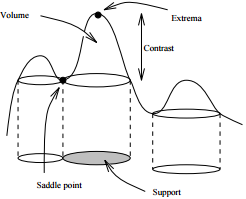
\includegraphics[width=0.35\textwidth]{fig/11.png}
    \vspace{-0.5em}   
    \begin{center}
    \caption{\textcolor{gray}{\footnotesize \textit{
    En blob visualiseret i 2-d, udefra Lindenberg's definition \cite{blob}}}}
    \label{fig:lindblob}
     \end{center}
  \end{figure}
       \vspace{-2.7em}
\noindent
%MEGA FORKERT
%MEGA FORKERT
%MEGA FORKERT
%MEGA FORKERT
I figur \ref{fig:lindblob}(a), ses en blob defineret af dens lokale ekstrema, hvor styrken af blobben beksrives ved kontrasten, ift. området omkring ekstremaet. Lindenberg definere en blob som værende afgrænset af dens saddelpunkt; et saddelpunkt angiver punktet, hvor intensiteten stopper med at falde og starter med at stige for lyse blobs, og modsat for mørke.
%MEGA FORKERT
%MEGA FORKERT
%MEGA FORKERT
%MEGA FORKERT
%MEGA FORKERT
%MEGA FORKERT
%MEGA FORKERT
\\
\\
En metode til at detektere ekstremaer, er Laplace af Gauss(LoG). Laplace defineres således:
\begin{equation}
\Delta f = \nabla^2 f =  \sum_{i = 1}^n \frac{\partial^2 f}{\partial x^2_i}
\end{equation}
Anvendes Laplace operatoren på Gaussfunktionen (ligning \eqref{2dgaussian}), kan resultatet diskretiseres og anvendes som en kerne.
\begin{equation}
LoG= \sigma^2\Delta G
\label{lap}
\end{equation}
Bemærk, at $\sigma^2$ er blevet multipliceret på fra venstre. Dette er gjort for at normalisere LoG, således, at responset er invariant overfor størrelsen af $\sigma$. LoG kan diskritiseres og foldes med billedet for at finde lokale ekstremaer. \\

\begin{figure}[H]
    \centering
    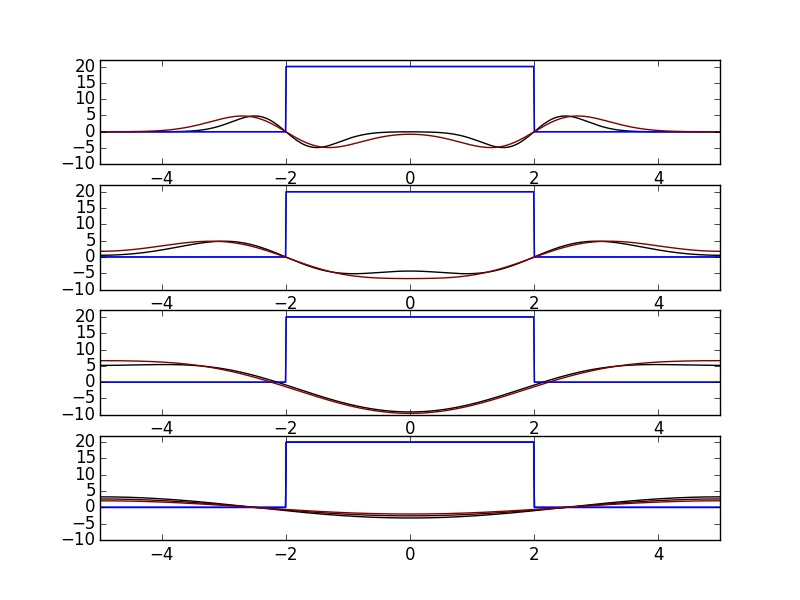
\includegraphics[width=0.90\textwidth]{fig/normLoG.jpg}
    \vspace{-0.5em}   
    \begin{center}
    \caption{\textcolor{gray}{\footnotesize \textit{
    (a) En 3-D visualisering af en to-dimensional Laplacian of Guassian (b) ét en-dimensionalt signal (c) Laplacian of Gaussian operatoren anvendt på (b)}}}
    \label{fig:normLoG}
     \end{center}
  \end{figure}
       \vspace{-2.5em}
\noindent
Når blobs skal lokaliseres, skal $\sigma$ værdien være tilpasses blobbens størrelse, som ses på figur \eqref{fig:normLoG}. Figuren viser fire forskellige værdier for $\sigma$. I første illustration er $\sigma$ værdien for lav - her dannes flere ekstremaer, men ingen af dem karakteriserer en blob, da den absolutte værdi for funktionen evalueret på det afledte af LoG signalet, er for lav. Dog ser kurven i illustration tre ud til, at have tilstrækkelig høj absolut værdi, til at kunne karakteriseres som et blob. \\
Problemet omkring valg af skala, kan afhjælpes ved skalarumsrepræsentation, som gennemgås i.

\begin{figure}[H]
    \centering
    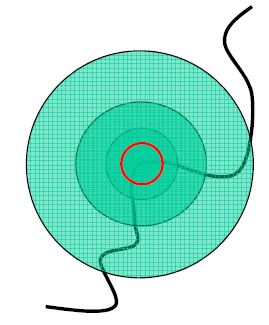
\includegraphics[width=0.25\textwidth]{fig/29.png}
    \vspace{-0.5em}   
    \begin{center}
    \caption{\textcolor{gray}{\footnotesize \textit{
    }}}
    \label{fig:scale}
     \end{center}
  \end{figure}
       \vspace{-2.5em}
\noindent
I figur \ref{fig:scale} angiver cirklerne forskellige undersøgte skalaer, Så hvordan udvælges cirklen, der dækker interesse området uafhængigt af områdets størrelse?  For Blobs er det interessant når der i et skaleret område opstår et veldefineret ekstrema. En måde at søge efter ekstremaer over forskellige skalaer er ved at oprette et skalarum for det undersøgte billede, hvor hvert billede skaleres og der for hver skala findes interessepunkter. Skala-rummet i et 2-dimensionalt billede repræsenteres af flere billeder i forskellige skalaer af det originale billede. Billeder, der repræsentere forskellige skalaer, opnås ved at folde billedet iterativt med et Gaussisk filter med stigende $\sigma$ værdi. 
\begin{figure}[H]
    \centering
    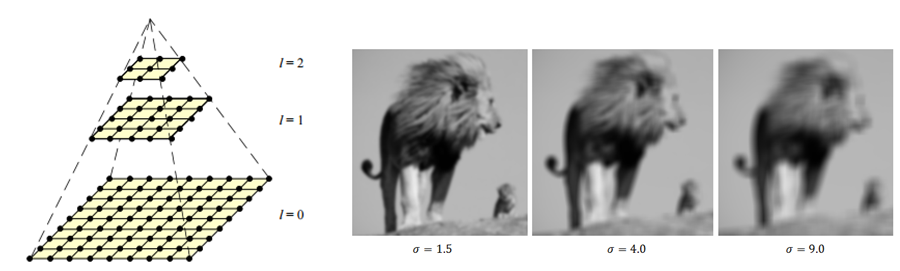
\includegraphics[width=0.65\textwidth]{fig/24.png}
    \vspace{-0.5em}   
    \begin{center}
    \caption{\textcolor{gray}{\footnotesize \textit{
Til venstre ses en visualisering af et skala-rum formet som en pyramide. Hvert niveau angiver en skala repræsentation af det originale vindue, hvor toppen af pyramiden indeholder billeder af største skala og derfor med mindst information, og bunden af skalaen med det originale billede. Til højre ses et billede foldet med et Gaussisk filter af stigende sigma værdier. Jo højere sigma værdi, jo flere fine detaljer bliver fjerne og billedet slørret.
    }}}
    \label{fig:mona}
     \end{center}
  \end{figure}
       \vspace{-2.5em}
\noindent
Et Gaussisk filter bruges da gradvis højere værdier af $\sigma$ fjerner fine strukturer, som vist i figur \ref{fig:mona}, og nye strukturer forekommer ikke ved transformationen fra finere til grovere skalaer \cite{lindenscale}. Idéen er derved at fjerne disse strukturer og lede efter  andre ekstremaer, gradvist på større skalaer, der også kan detekteres.
Et billede i skalarummet for billedet $f(x,y)$ kan derfor defineres som i \eqref{scalespace}
\begin{equation}
L(x,y,\sigma) = G(x,y,\sigma)\ast f(x,y)
\label{scalespace}
\end{equation}
hvor $G$ er det 2-dimensionelle Gaussiske filter,$L(x,y,\sigma)$ repræsentere et et billede i skala-rummet, og skala-parametren $\sigma$, bestemmer skalaen, eller placeringen i skala-rummet. $L(x,y,0) = f(x,y)$, da det er den "nederste" skala og den nederste del af pyramiden. Højere niveauer af pyramiden kan opnås ved at folde billedet med et Gaussisk filter af større sigma værdi.